\documentclass{article}[11pt]
\usepackage{graphicx}
\usepackage{amsmath,amsfonts}

\title{Dot Products and Cosines}

\begin{document}

\maketitle

\section{Dot Products}
The \emph{dot product} of two vectors $a, b \in \mathbb{R}^n$ is the sum of the products of their components:

\[ a \cdot b = \sum_{i=0}^{n-1} a_i b_i \]

The dot product is related to the length of a vector by the Pythagorean theorem:

\begin{equation}
\label{eqn:pythagorean}
|a|^2 = a \cdot a
\end{equation}

It is a well known fact that the geometric interpretation of the dot product is that it is the cosine of the angle between the pair of vectors scaled by their lengths:

\begin{equation}
\label{eqn:dotprodcos}
a \cdot b = |a| |b| \cos(\theta)
\end{equation}

From a certain perspective this can be taken to be the defining property of the cosine (as is commonly done in more advanced treatments).  However, that is not the approach adopted in this document.  Instead we will derive Eqn.~\ref{eqn:dotprodcos} from the principles of trigonometry and Euclidean geometry.

\section{Proof of the Dot Product Cosine Rule}
Consider the length of the difference between $a$ and $b$.  Using Eqn.~\ref{eqn:pythagorean}:

\begin{equation}
\label{eqn:simpledist}
|a - b|^2 = a \cdot a - 2 a \cdot b + b \cdot b
\end{equation}

Now let us derive this quantity in a different way, starting from the following picture:

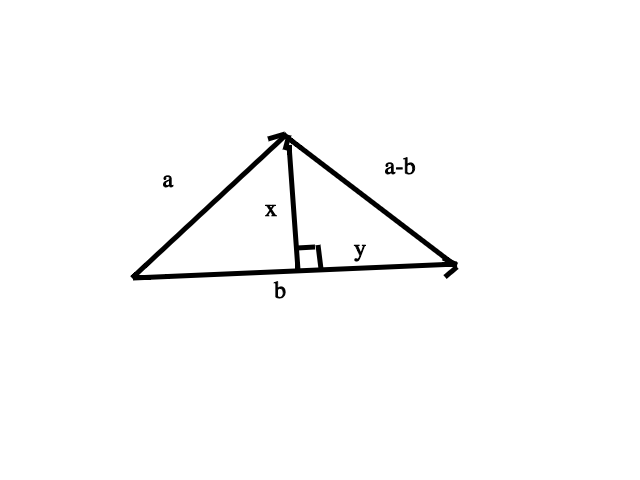
\includegraphics[width=4in]{triangle.png}

Again using the Pythagorean theorem, we can conclude that:

\begin{equation}
\label{eqn:righttri}
|a - b|^2 = |x|^2 + |y|^2
\end{equation}

Using trigonometry we can see that:

\begin{eqnarray*}
|x| & = & |a| \sin(\theta) \\
|y| & = & |b| - |a| \cos(\theta)
\end{eqnarray*}

Subsituting back into Eqn.~\ref{eqn:righttri} gives:

\begin{eqnarray*}
|a - b|^2  & = & |a|^2 \sin(\theta)^2 + |a|^2 \cos(\theta)^2 - 2 |a| |b| \cos(\theta) + |b|^2 \\
& = & |a|^2 - 2 |a| |b| \cos(\theta) + |b|^2
\end{eqnarray*}

Now we apply Eqn.~\ref{eqn:simpledist}, and see that:

\[  a \cdot a - 2 a \cdot b + b \cdot b = |a|^2 - 2 |a| |b| \cos(\theta) + |b|^2 \]

And applying Eqn.~\ref{eqn:pythagorean} again shows that:

\[ a \cdot b = |a| |b| \cos(\theta) \]

Which completes the proof Eqn.~\ref{eqn:dotprodcos}.

\section{Proof using complex numbers}
There is a second way to prove Eqn.~\ref{eqn:dotprodcos} in 2D using complex numbers and Euler's formula:
\[ e^{i \theta} = \cos(\theta) + i \sin(\theta) \]

To do this, we first represent the vectors $a$ and $b$ as complex numbers:

\begin{eqnarray*}
a & = & a_x + a_y i \\
b & = & b_x + b_y i
\end{eqnarray*}

Then,

\[ a \overline{b} = (a_x + a_y i)(b_x - b_y i) \]

And so,

\begin{equation}
\label{eqn:cartesian}
a \overline{b} =  a_x b_x + a_y b_y + (a_y b_x - a_x b_y) i
\end{equation}

On the other hand, we can also write $a$ and $b$ in polar coordinates:

\begin{eqnarray*}
a & = & a_r e^{i a_\theta} \\
b & = & b_r e^{i b_\theta}
\end{eqnarray*}

And,

\begin{equation}
\label{eqn:polar}
a \overline{b} = a_r b_r e^{i (a_\theta - b_\theta)}
\end{equation}

Now observe that:

\begin{eqnarray*}
|a| & = & a_r \\
|b| & = & b_r \\
\theta & = & a_\theta - b_\theta
\end{eqnarray*}

And set Eqn.~\ref{eqn:polar} equal to Eqn.~\ref{eqn:cartesian} giving,

\begin{equation}
a_x b_x + a_y b_y + (a_y b_x - a_x b_y) i = |a| |b| \cos(\theta) + |a| |b| \sin(\theta) i
\end{equation}

Splitting this equation up into real and imaginary parts gives the following identities:

\begin{eqnarray}
\label{eqn:complexdot} a_x b_x + a_y b_y & = & |a| |b| \cos(\theta) \\
\label{eqn:complexperp} a_y b_x - a_x b_y & = & |a| |b| \sin(\theta)
\end{eqnarray}

And so Eqn.~\ref{eqn:complexdot} proves the dot product formula for 2D.  The second equation, Eqn.~\ref{eqn:complexperp} is known as the \emph{perpendicular product formula} and is a special case of a determinant identity.

\end{document}